\documentclass[a4paper]{article} 
\usepackage{graphicx} 
\usepackage[ngerman]{babel} 
\usepackage[ansinew]{inputenc} 
\usepackage[T1]{fontenc} 
\usepackage{tgpagella} 
\usepackage{geometry} 
\usepackage{color} 
\usepackage{microtype} 
\usepackage{minted}
\usepackage{caption}
\usepackage[headsepline,footsepline]{scrpage2}
\usepackage{textcomp}
\usepackage{pdfpages}
\usepackage{mdframed}



\makeatletter
\renewcommand\minted@pygmentize[2][\jobname.pyg]{
  \def\minted@cmd{pygmentize -l #2 -f latex -F tokenmerge
    \minted@opt{gobble} \minted@opt{texcl} \minted@opt{mathescape}
    \minted@opt{startinline} \minted@opt{funcnamehighlighting}
    \minted@opt{linenos} -P "verboptions=\minted@opt{extra}"
    -O encoding=UTF-8,outencoding=iso-8859-1 -o \jobname.out.pyg #1}
  \immediate\write18{\minted@cmd}
  % For debugging, uncomment:
  %\immediate\typeout{\minted@cmd}
  \ifthenelse{\equal{\minted@opt@bgcolor}{}}
   {}
   {\begin{minted@colorbg}{\minted@opt@bgcolor}}
  \input{\jobname.out.pyg}
  \ifthenelse{\equal{\minted@opt@bgcolor}{}}
   {}
   {\end{minted@colorbg}}
  \DeleteFile{\jobname.out.pyg}}
\makeatother


\title{Dokumentation - 6 Übung}
\author{Roman Lumetsberger}
\date{\today}

\newmintedfile[ccode]{cpp}{
               linenos,
               numbersep=5pt,
               frame=lines,
               framesep=2mm
}

\newmintedfile[javacode]{java}{
               linenos,
               numbersep=5pt,
               frame=lines,
               tabsize=2,
               framesep=2mm,
}
\newmintedfile[csscode]{css}{
               linenos,
               numbersep=5pt,
               frame=lines,
               tabsize=2,
               framesep=2mm,
}
\newmintedfile[sqlcode]{sql}{
               linenos,
               numbersep=5pt,
               frame=lines,
               tabsize=2,
               framesep=2mm,
}
\captionsetup{
  font=footnotesize,
  justification=raggedright,
  singlelinecheck=false
}


\newcommand{\srcDir}{../Beispiel/src/at/lumetsnet/caas/}
\newcommand{\testDir}{../Beispiel/test/at/lumetsnet/caas/test/}

\definecolor{lineColor}{RGB}{151,0,0}
\pagestyle{scrheadings}
\clearscrheadfoot
\begin{document}
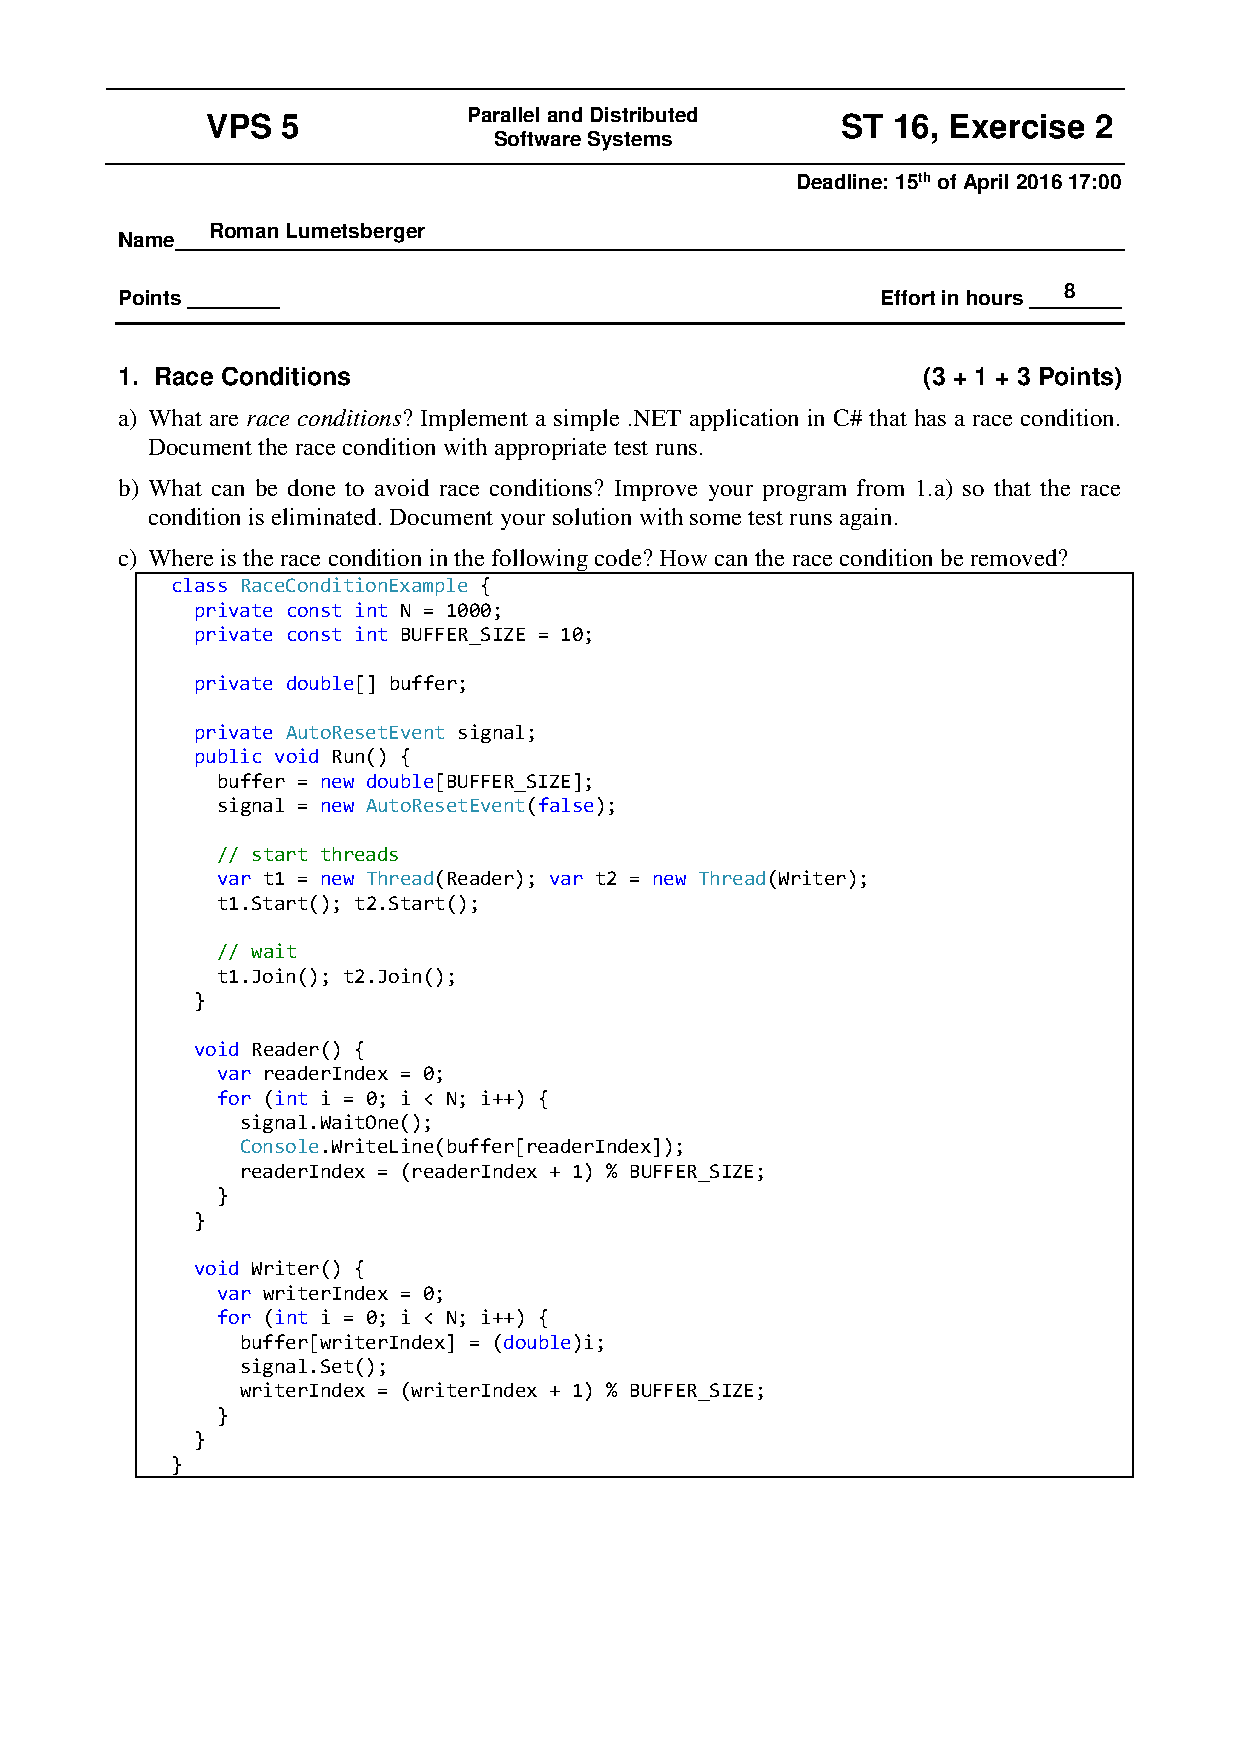
\includepdf[pages=-]{angabe.pdf}

\ihead{VPS SS 2016 - �bung 02}
\ifoot{Roman Lumetsberger}
\cfoot{1310307026}
\ofoot{Seite \pagemark}

\section{Race Conditions}
\subsection*{1a. Was sind race conditions?}
\textbf{Race conditions} k�nnen entstehen, wenn mehrere Threads paralell auf den selben Speicherbereich (Variable) zugreifen und ver�ndern. Das Ergebnis ist abh�ngig von der zeitlichen Abfolge der Threads und somit nicht vorhersehbar.
\begin{figure}[!htb]
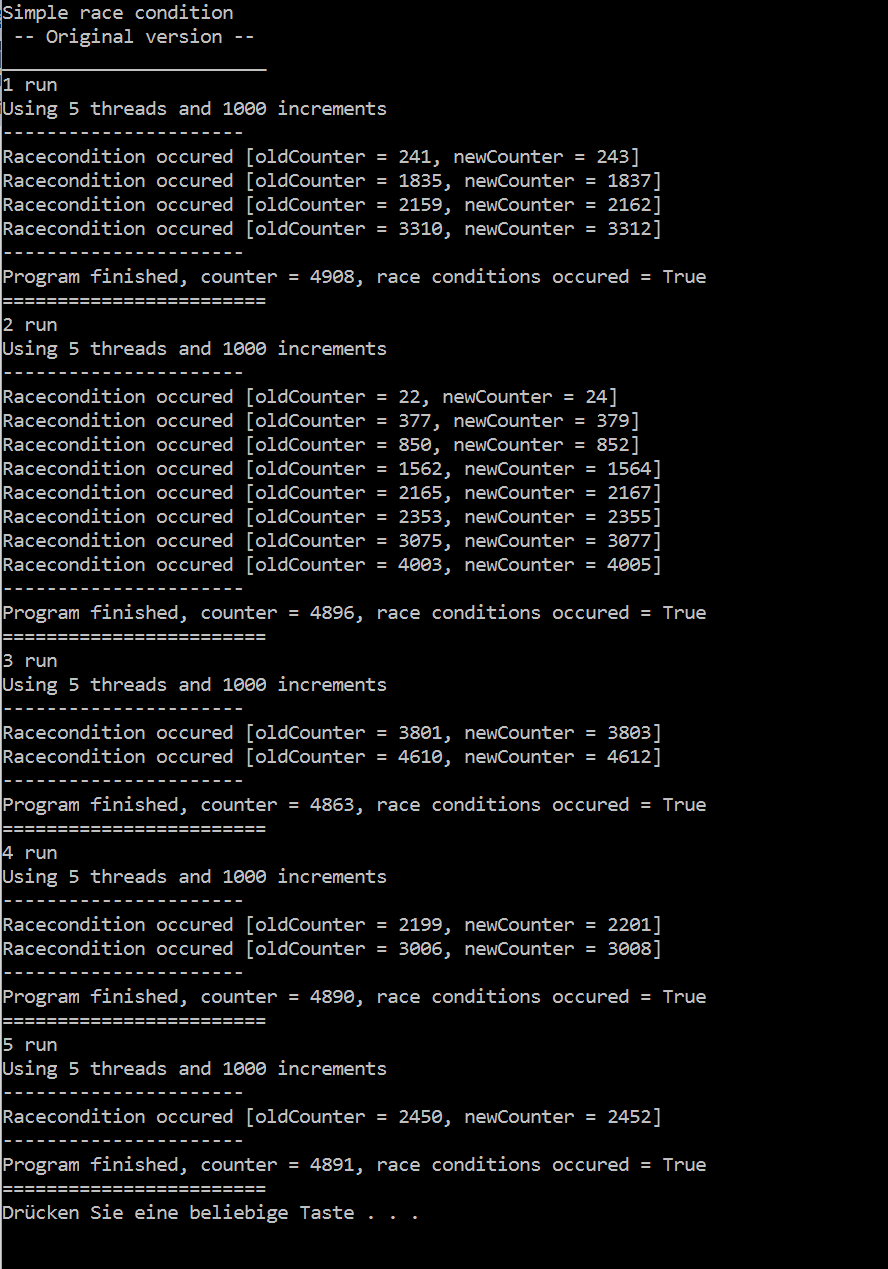
\includegraphics[width=300px]{images/1a.png}
\caption{Race codition in CSharp - Original version}
\label{fig:SimpleRaceConditionOriginal}
\end{figure}

Abbildung~\ref{fig:SimpleRaceConditionOriginal} zeigt die Ausgabe der implementierten race codition in CSharp. Dabei wird eine Variable \texttt{\_counter} erh�ht und dann mit dem vorherigen Wert verglichen. Der neue Wert sollte genau um eins gr��er sein als der alte Wert. Ist dies nicht der Fall ist eine race condition aufgetreten. Die Variable wurde also von einem anderen Thread ge�ndert.

\subsection*{1b. Wie k�nnen race conditions vermieden werden?}
Diese k�nnen mit Hilfe von Locks vermieden werden.
\begin{figure}[!htb]
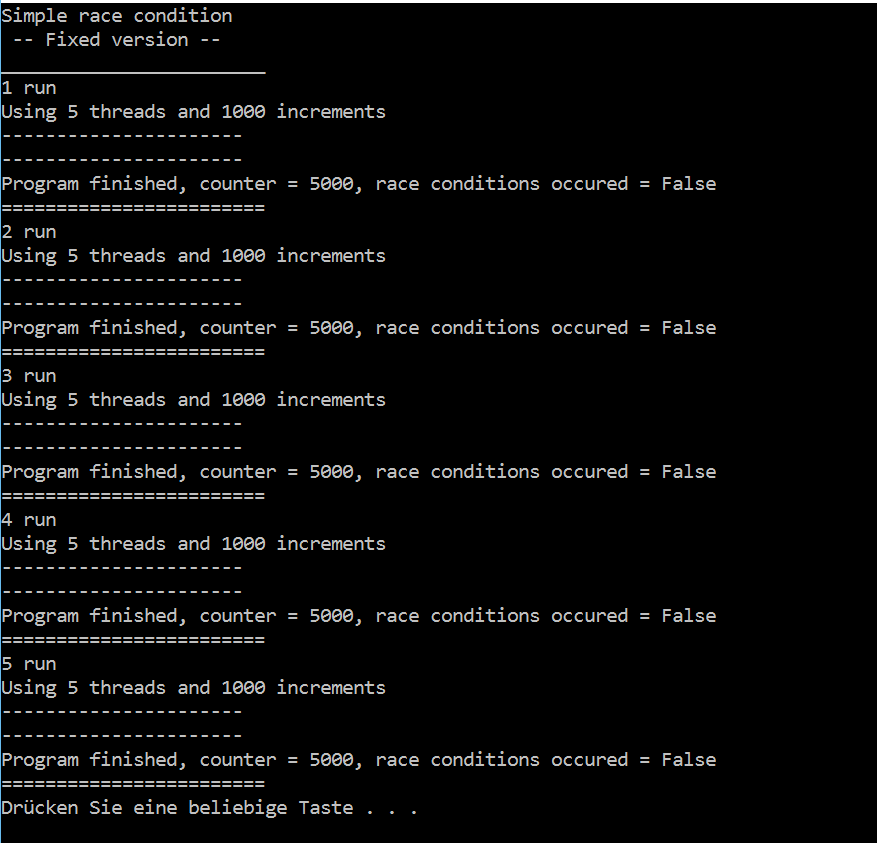
\includegraphics[width=300px]{images/1b.png}
\caption{Race condition in CSharp - Ohne race condition}
\label{fig:SimpleRaceConditionFixed}
\end{figure}

Abbildung~\ref{fig:SimpleRaceConditionFixed} zeigt die Ausgabe der verbesserten Version. Diese verwendet Locks um die race condition zu vermeiden.

\subsection*{1c. Race condition im Code}
Die race condition im angegebenen Code ist die Tatsache, das das der Writer und Reader nicht korrekt miteinander synchronisiert sind und nur ein begrenzter Puffer zur Verf�gung steht. Dadurch kann es sein, dass der Writer bereits mehr Werte erzeugt als der Puffer zul�sst und somit die alten Werte �berschreibt.
Die L�sung ist die korrekte Synchronisation der beiden Threads.
\cscode{\srcDir/RaceConditionExample/RaceConditionExample.cs}

\section{Synchronization Primitives}
\subsection*{2a. / 2b.}
\cscode{\srcDir/SynchronizationPrimitives/LimitedConnectionsExample.cs}
\subsection*{2c. Aktives Warten}
 \cscode{\srcDir/SynchronizationPrimitives/PollingExample.cs}

\section{Toilet Simulation}
\subsection*{3a. Toilet Implementierung}
Diese Aufgabe wurde bereits in der �bung gemacht. Der \texttt{Consumer} ist fertig, wenn alle Elemente der Warteschlange abgearbeitet sind. Dazu wurde das Interface \texttt{IQueue} um das Property \texttt{IsCompleted} erweitert.

Die Synchronisation wurde ebenfalls �ber die Warteschlange gel�st. Hier wurde ebenfalls das Interface \texttt{IQueue} um die Methode \texttt{TryDequeue} erweitert. Diese blockiert, falls aktuell kein Element vorhanden ist.

\subsection*{3b. FifoQueue Implementierung}
Die \texttt{FifoQueue} wurde mit Hilfe einer Semaphore implementiert. Dabe wird bei jedem \texttt{Enqueue} die Semaphore um eins erh�ht und beim \texttt{TryDequeue} wird diese wieder veringert. Damit wird der gew�nschte Effekt erreicht, das die Methode \texttt{TryDequeue} blockiert. Dabei kann es sein, dass die Queue bereits leer ist und trotzdem noch Threads in der Methode \texttt{TryDequeue} auf Elemente warten. Um das Warten zu beenden wurde ein \texttt{CancellationToken} verwendet, der beim \texttt{Wait} mitgegeben wird. Damit k�nnen diese Threads aufgeweckt und beendet werden. Um race conditions zu vermeiden wurde jeder Zugriff auf den Datenspeicher mit Locks gesch�tzt.

 

\end{document}